\documentclass{article}
\usepackage[margin = 1in]{geometry}
\usepackage{tcolorbox}
\usepackage{enumerate}
\usepackage{ragged2e}
\usepackage{amsmath}
\usepackage{amssymb}
\usepackage{fancyhdr}
\usepackage{subfig}
\usepackage{epstopdf}
\usepackage{xcolor}
\usepackage{dsfont}
\usepackage[justification=centering]{caption}

\renewcommand{\vec}[1]{\mathbf{#1}}
\newcommand{\qed}{\hfill$\blacksquare$}
\newcommand{\var}{\mathrm{Var}}

\begin{document}

\RaggedRight
\pagestyle{fancy}

\rhead{\footnotesize\uppercase{16-831: Statistical Techniques in Robotics}} 

{\large Project 2: Multi-Armed Bandits} \\[0.5\parsep]
Dawei Wang (daweiwan@andrew.cmu.edu)

\begin{itemize}

	\begin{figure}[b!]
		\centering
		\includegraphics[width = \textwidth]{images/plot25.eps}
		\caption{Constant Policy and Random Policy versus Constant Game}
		\label{plot25}
	\end{figure}	

	\item 2.5: See Figure \ref{plot25}. 

	\begin{figure}[b!]
		\centering
		\includegraphics[width = \textwidth]{images/plot311.eps}
		\caption{Generalized Weighted Majority (GWM) versus Constant Game}
		\label{plot311}
	\end{figure}	

	\item 3.1.1: The regret grows linearly. This is anticipated because the selected action	
		is always penalized, and the other action is not penalized if not selected.
		Each time this happens, the expected action will move towards the other action;
		after a certain number of iterations, the other action will be favored, resulting 
		in a substantial loss, which in turn penalizes this inferior action and makes
		the expected action rewind to the superior action again. This cycle repeats 
		infinitely. In our scenario, the losses are 0.2 and 0.8 respectively; the expected
		action in each cycle would be 1, 1, 1, 1, 2, since $0.2\times4=0.8\times1$, equivalent
		to having an average reward of $(0.8\times4+0.2\times1)\div5=0.68$, which explains the
		observed regret $\tilde{R}=120=0.8\times1000-0.68\times1000$ in Figure \ref{plot311}.
	
	\item 3.1.2: It is yet unclear why the regret bound would be substantially higher. 
	\begin{equation}
		\bar{R}_n=\mathbb{E}\sum_{t=1}^nl_{I_t,t}-\min_{i=1,\dots,K}\mathbb{E}\sum_{t=1}^nl_i,t
	\end{equation}
		
	\item 3.1.3: The statement is true because 
	\begin{equation}
		E\left[\sum_{t=1}^T\tilde{l}_n^t\right]=\sum_{t=1}^T
		E\left[\frac{l_n^t}{p_n^t}\mathds{1}_{a^t=n}\right]=\sum_{t=1}^T
		\left[\frac{l_n^t}{p_n^t}p(a^t=n)+0\cdot p(a^t\ne n)\right]=\sum_{t=1}^T
		\frac{l_n^t}{p_n^t}p_n^t=\sum_{t=1}^Tl_n^t
	\end{equation}
	
	\begin{figure}[t!]
		\centering
		\includegraphics[width = \textwidth]{images/plot321.eps}
		\caption{Exponential Weights for Exploration and Exploitation (EXP3) versus Constant Game}
		\label{plot321}
	\end{figure}		
	
	\item 3.2.1:	See Figure \ref{plot321}. EXP3 penalizes the inferior action
		super-exponentially by first lowering the probability of it being selected, 
		and then amplifying the penalty by dividing the loss by the already small 
		probability, in the rare case that it is indeed selected again. It would
		therefore take a considerable number of iterations for the probability of
		the superior action to drop to a similar level, causing the inferior action
		to be selected once and it being penalized further significantly. Generally,
		in the case of playing a constant game, the superior action can be quickly identified. 
		
	\begin{figure}[t!]
		\centering
		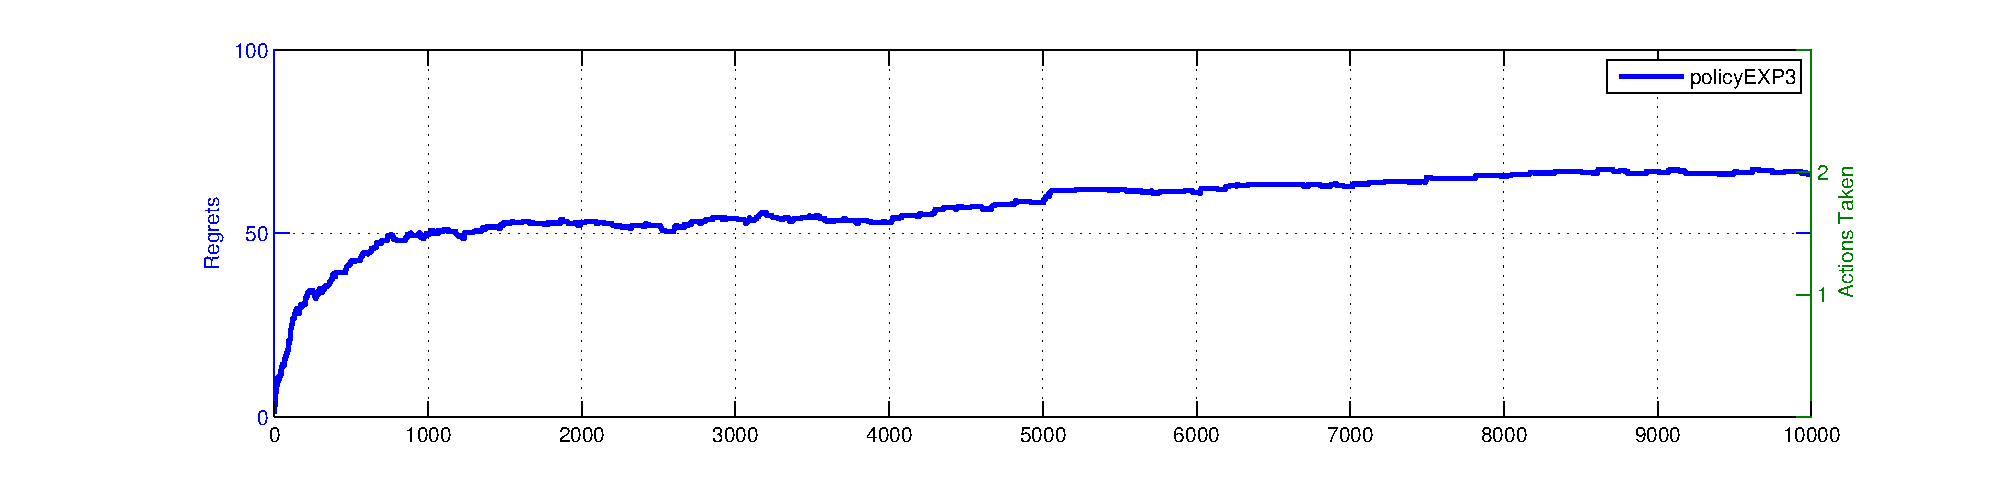
\includegraphics[width = \textwidth]{images/plot332.eps}
		\caption{Exponential Weights for Exploration and Exploitation (EXP3) versus Gaussian Game}
		\label{plot332}
	\end{figure}		
		
	\item 3.3.2: See Figure \ref{plot332}.
		
	\item 3.4.1: The variance is unbounded since
	\begin{flalign}
		\var\left[\sum_{t=1}^T\tilde{l}_n^t\right]&=
			E\left[\left(\sum_{t=1}^T\tilde{l}_n^t\right)^2\right]+
			\left(E\left[\sum_{t=1}^T\tilde{l}_n^t\right]\right)^2\\
		&=E\left[\left(\sum_{t=1}^T\frac{l_n^t}{p_n^t}\mathds{1}_{a_t=n}\right)^2\right]+
			\left(\sum_{t=1}^T l_n^t\right)^2\\
		&=E\left[\sum_{t=1}^T\left(\frac{l_n^t}{p_n^t}\mathds{1}_{a_t=n}\right)^2\right]
			+E\left[\sum_{t_1}^T\sum_{t_2\ne t_1}^T
			\left(\frac{l_n^{t_1}}{p_n^{t_1}}\mathds{1}_{a_{t_1}=n}\right)
			\left(\frac{l_n^{t_2}}{p_n^{t_2}}\mathds{1}_{a_{t_2}=n}\right)
			\right]+\left(\sum_{t=1}^T l_n^t\right)^2\\
		&=\sum_{t=1}^T\left(\frac{l_n^t}{p_n^t}\right)^2p_n^t+
			\sum_{t_1}^T\sum_{t_2\ne t_1}^Tl_n^{t_1}l_n^{t_2}
			\frac{P(a_{t_1}=n,a_{t_2}=n)}{p_n^{t_1}p_n^{t_2}}+\left(\sum_{t=1}^T l_n^t\right)^2.
	\end{flalign}
	Here even if the loses are bounded, the probability that appears on the denominator of
	the first term can be infinitely close to zero, such that the first term is unbounded.
	Although the probability also appears on the denominator of the second term, but due to 
	its nominator this term is not necessarily unbounded; it is written as-is because those
	two events are not necessarily independent. This does not affect our conclusion that
	the variance is unbounded though. The third term is always bounded. 
	
	\item 4.2.1: It is straightforward to see that, using the Hoeffding's Inequality, 
	\begin{equation}
		P\left(\left|\mu-\hat{\mu}\right|\ge\sqrt{\frac{\log(\delta^{-1})}{2m}}\right)
		\le\exp\left[-2m\left(\sqrt{\frac{\log(\delta^{-1})}{2m}}\right)^2\right]=\delta
	\end{equation}
	which indicates that the probability that $\mu\ge\hat{\mu}+\sqrt{(\log(\delta^{-1}))/2m}$
	is at most $\delta$, which is equivalent in saying that the probability that 
	$\mu\le\hat{\mu}+\sqrt{(\log(\delta^{-1}))/2m}$ is at least $1-\delta$. 
	
	\item 4.2.2: Using the conclusion from 4.2.1, and considering the fact that
	$C_n^t$ is the number of times that the reward is sampled, we have $m=C_n^t$, 
	and $\delta^{-1}=t$, which trivially yields
	\begin{equation}
		\mu_n^t\le\hat{\mu}_n^t+\sqrt{\frac{\log t}	{2C_n^t}}
		\label{ucb}
	\end{equation}
	
	\begin{figure}[b!]
		\centering
		\includegraphics[width = \textwidth]{images/plot431-wucb.eps}
		\caption{Upper Confidence Bound (UCB) versus Constant Game}
		\label{plot431}
	\end{figure}
	
	\item 4.3.1: See Figure \ref{plot431}. Note that the actions taken are not plotted
		since it is straightforward to see that the inferior action is taken whenever
		the regret steps up, and the superior action otherwise. In the case of playing
		a constant game, the estimated rewards for both actions converge to their true
		values almost immediately; the superior action will then always be selected 
		since it has higher reward, until $C_2^t$ on the denominator of the second term
		is large enough and compensate for the reward difference. This causes the inferior
		action to be taken, which increments $C_1^t$ and requires $C_2^t$ to be again
		adequately large in order to toggle the selected action. This happens each time
		the upper confidence bounds meet on the plot. This can be numerically solved: 
		\begin{equation}
			\sqrt{\frac{\log(C_1^t+C_2^t)}{2C_1^t}}+0.2=
			\sqrt{\frac{\log(C_1^t+C_2^t)}{2C_2^t}}+0.8
		\end{equation}
		for $C_1^t=1,2,3,\dots,6,7$, we can obtain solutions for
		$C_2^t=6,20,46,93,176,322,575$, which are basically where the inferior 
		action is taken. 
	
	\begin{figure}[b!]
		\centering
		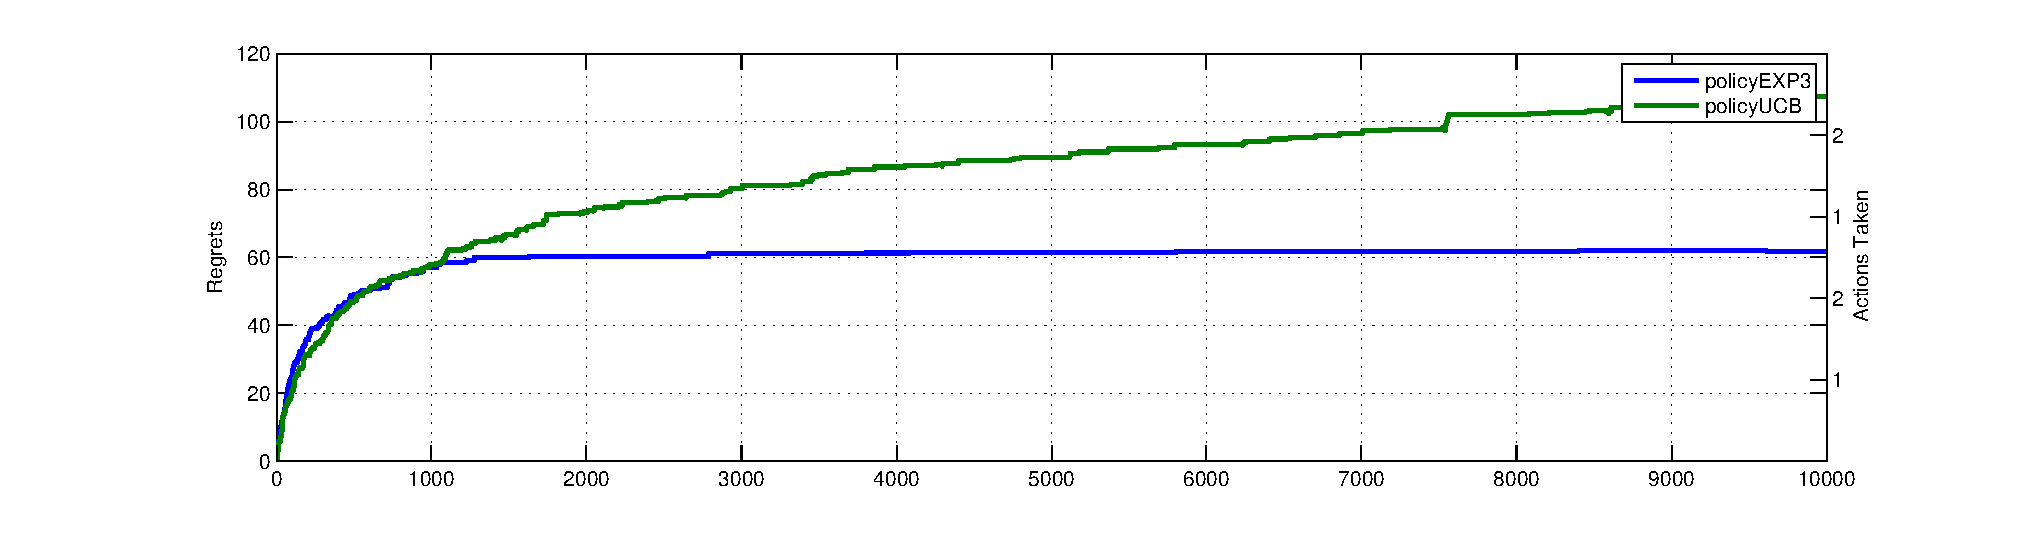
\includegraphics[width = \textwidth]{images/plot441.eps}
		\caption{UCB and EXP3 versus Gaussian Game}
		\label{plot441}
	\end{figure}
	
	\item 4.4.1: See Figure \ref{plot441}. UCB outperforms EXP3 initially, but the 
		regret for EXP3 quickly approaches some asymptotic bound while that for 
		UCB continues to grow. This is anticipated since the estimator for EXP3
		is unbiased; it converges quickly to the true mean rewards for each action
		and all subsequent actions sampled from that multinomial distribution will
		truly reflect the expected rewards from both actions. However, Although 
		UCB is able to converge to the true mean rewards equally well, its upper
		confidence bounds for the better actions almost monotonically decrease and the 
		worse actions are guaranteed to be selected from time to time. 
		
	\begin{figure}[h]
		\centering
		\includegraphics[width = \textwidth]{images/plot451.eps}
		\caption{UCB and EXP3 versus Adversarial Game}
		\label{plot451}
	\end{figure}	
	
	\item 4.5.1: See Figure \ref{plot451}. The adversarial game uses the following reward table:
	\begin{equation}
		\begin{bmatrix}0&1&0&1&0&1&0&1&\dots&1\\
		1&0&1&0&1&0&1&0&\dots&0\end{bmatrix}
	\end{equation}
	In the first iteration, UCB simply chooses the first action since it possesses zero
	knowledge on any of the actions; it then realizes that no reward is incurred for taking
	this action and consequently goes on to explore the second action, which also results
	in zero reward. UCB can do nothing at this point except for repetitively exploring
	alternating actions only to achieve zero reward. It is straightforward to see that
	the best action results in a reward of 500. This can also be generalized: if there
	are $n$ actions, the regret would be $1000\cdot (n-1)/n$. EXP3 takes advantage of 
	randomization and is more robust against an adversarial game. 
	
	\item 5.2.1: See Figure \ref{plot521}. 
	\item 5.3.1: See Figure \ref{plot531}.
	
\end{itemize}	

\begin{figure}[h]
	\centering
	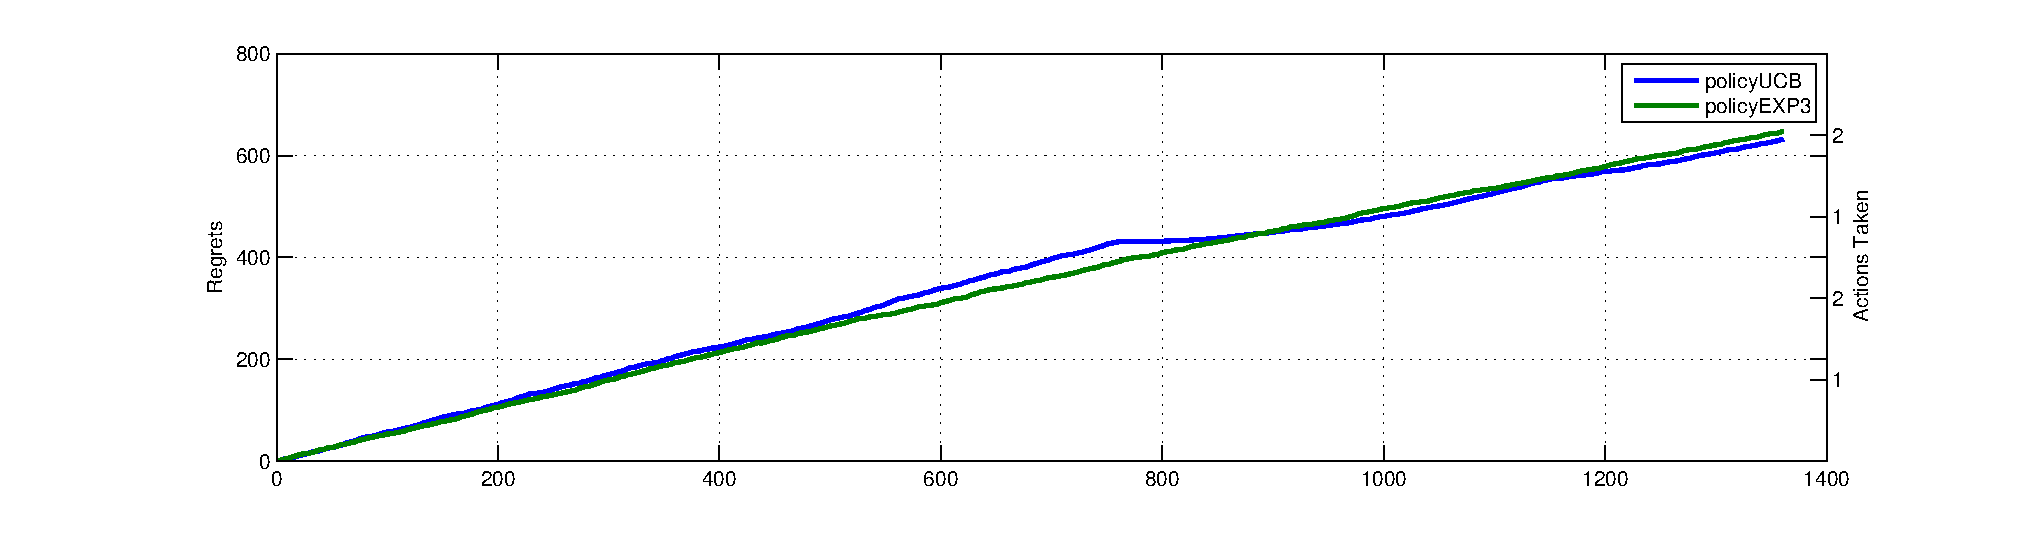
\includegraphics[width = 0.9\textwidth]{images/plot521.eps}
	\caption{UCB and EXP3 on the University Website Latency Dataset}
	\label{plot521}
\end{figure}

\begin{figure}[h]
	\centering
	\includegraphics[width = 0.9\textwidth]{images/plot531.eps}
	\caption{UCB and EXP3 on the Path Planning Dataset}
	\label{plot531}
\end{figure}


		
\end{document}